% Options for packages loaded elsewhere
\PassOptionsToPackage{unicode}{hyperref}
\PassOptionsToPackage{hyphens}{url}
%
\documentclass[
  a4paper,
]{article}
\usepackage{amsmath,amssymb}
\usepackage{lmodern}
\usepackage{iftex}
\ifPDFTeX
  \usepackage[T1]{fontenc}
  \usepackage[utf8]{inputenc}
  \usepackage{textcomp} % provide euro and other symbols
\else % if luatex or xetex
  \usepackage{unicode-math}
  \defaultfontfeatures{Scale=MatchLowercase}
  \defaultfontfeatures[\rmfamily]{Ligatures=TeX,Scale=1}
\fi
% Use upquote if available, for straight quotes in verbatim environments
\IfFileExists{upquote.sty}{\usepackage{upquote}}{}
\IfFileExists{microtype.sty}{% use microtype if available
  \usepackage[]{microtype}
  \UseMicrotypeSet[protrusion]{basicmath} % disable protrusion for tt fonts
}{}
\makeatletter
\@ifundefined{KOMAClassName}{% if non-KOMA class
  \IfFileExists{parskip.sty}{%
    \usepackage{parskip}
  }{% else
    \setlength{\parindent}{0pt}
    \setlength{\parskip}{6pt plus 2pt minus 1pt}}
}{% if KOMA class
  \KOMAoptions{parskip=half}}
\makeatother
\usepackage{xcolor}
\IfFileExists{xurl.sty}{\usepackage{xurl}}{} % add URL line breaks if available
\IfFileExists{bookmark.sty}{\usepackage{bookmark}}{\usepackage{hyperref}}
\hypersetup{
  pdftitle={MATH3714 Linear Regression and Robustness},
  pdfauthor={Jochen Voss},
  hidelinks,
  pdfcreator={LaTeX via pandoc}}
\urlstyle{same} % disable monospaced font for URLs
\usepackage[margin=1in]{geometry}
\usepackage{color}
\usepackage{fancyvrb}
\newcommand{\VerbBar}{|}
\newcommand{\VERB}{\Verb[commandchars=\\\{\}]}
\DefineVerbatimEnvironment{Highlighting}{Verbatim}{commandchars=\\\{\}}
% Add ',fontsize=\small' for more characters per line
\usepackage{framed}
\definecolor{shadecolor}{RGB}{248,248,248}
\newenvironment{Shaded}{\begin{snugshade}}{\end{snugshade}}
\newcommand{\AlertTok}[1]{\textcolor[rgb]{0.94,0.16,0.16}{#1}}
\newcommand{\AnnotationTok}[1]{\textcolor[rgb]{0.56,0.35,0.01}{\textbf{\textit{#1}}}}
\newcommand{\AttributeTok}[1]{\textcolor[rgb]{0.77,0.63,0.00}{#1}}
\newcommand{\BaseNTok}[1]{\textcolor[rgb]{0.00,0.00,0.81}{#1}}
\newcommand{\BuiltInTok}[1]{#1}
\newcommand{\CharTok}[1]{\textcolor[rgb]{0.31,0.60,0.02}{#1}}
\newcommand{\CommentTok}[1]{\textcolor[rgb]{0.56,0.35,0.01}{\textit{#1}}}
\newcommand{\CommentVarTok}[1]{\textcolor[rgb]{0.56,0.35,0.01}{\textbf{\textit{#1}}}}
\newcommand{\ConstantTok}[1]{\textcolor[rgb]{0.00,0.00,0.00}{#1}}
\newcommand{\ControlFlowTok}[1]{\textcolor[rgb]{0.13,0.29,0.53}{\textbf{#1}}}
\newcommand{\DataTypeTok}[1]{\textcolor[rgb]{0.13,0.29,0.53}{#1}}
\newcommand{\DecValTok}[1]{\textcolor[rgb]{0.00,0.00,0.81}{#1}}
\newcommand{\DocumentationTok}[1]{\textcolor[rgb]{0.56,0.35,0.01}{\textbf{\textit{#1}}}}
\newcommand{\ErrorTok}[1]{\textcolor[rgb]{0.64,0.00,0.00}{\textbf{#1}}}
\newcommand{\ExtensionTok}[1]{#1}
\newcommand{\FloatTok}[1]{\textcolor[rgb]{0.00,0.00,0.81}{#1}}
\newcommand{\FunctionTok}[1]{\textcolor[rgb]{0.00,0.00,0.00}{#1}}
\newcommand{\ImportTok}[1]{#1}
\newcommand{\InformationTok}[1]{\textcolor[rgb]{0.56,0.35,0.01}{\textbf{\textit{#1}}}}
\newcommand{\KeywordTok}[1]{\textcolor[rgb]{0.13,0.29,0.53}{\textbf{#1}}}
\newcommand{\NormalTok}[1]{#1}
\newcommand{\OperatorTok}[1]{\textcolor[rgb]{0.81,0.36,0.00}{\textbf{#1}}}
\newcommand{\OtherTok}[1]{\textcolor[rgb]{0.56,0.35,0.01}{#1}}
\newcommand{\PreprocessorTok}[1]{\textcolor[rgb]{0.56,0.35,0.01}{\textit{#1}}}
\newcommand{\RegionMarkerTok}[1]{#1}
\newcommand{\SpecialCharTok}[1]{\textcolor[rgb]{0.00,0.00,0.00}{#1}}
\newcommand{\SpecialStringTok}[1]{\textcolor[rgb]{0.31,0.60,0.02}{#1}}
\newcommand{\StringTok}[1]{\textcolor[rgb]{0.31,0.60,0.02}{#1}}
\newcommand{\VariableTok}[1]{\textcolor[rgb]{0.00,0.00,0.00}{#1}}
\newcommand{\VerbatimStringTok}[1]{\textcolor[rgb]{0.31,0.60,0.02}{#1}}
\newcommand{\WarningTok}[1]{\textcolor[rgb]{0.56,0.35,0.01}{\textbf{\textit{#1}}}}
\usepackage{longtable,booktabs,array}
\usepackage{calc} % for calculating minipage widths
% Correct order of tables after \paragraph or \subparagraph
\usepackage{etoolbox}
\makeatletter
\patchcmd\longtable{\par}{\if@noskipsec\mbox{}\fi\par}{}{}
\makeatother
% Allow footnotes in longtable head/foot
\IfFileExists{footnotehyper.sty}{\usepackage{footnotehyper}}{\usepackage{footnote}}
\makesavenoteenv{longtable}
\usepackage{graphicx}
\makeatletter
\def\maxwidth{\ifdim\Gin@nat@width>\linewidth\linewidth\else\Gin@nat@width\fi}
\def\maxheight{\ifdim\Gin@nat@height>\textheight\textheight\else\Gin@nat@height\fi}
\makeatother
% Scale images if necessary, so that they will not overflow the page
% margins by default, and it is still possible to overwrite the defaults
% using explicit options in \includegraphics[width, height, ...]{}
\setkeys{Gin}{width=\maxwidth,height=\maxheight,keepaspectratio}
% Set default figure placement to htbp
\makeatletter
\def\fps@figure{htbp}
\makeatother
\setlength{\emergencystretch}{3em} % prevent overfull lines
\providecommand{\tightlist}{%
  \setlength{\itemsep}{0pt}\setlength{\parskip}{0pt}}
\setcounter{secnumdepth}{5}
\ifLuaTeX
  \usepackage{selnolig}  % disable illegal ligatures
\fi
\usepackage[]{natbib}
\bibliographystyle{plainnat}

\title{MATH3714 Linear Regression and Robustness}
\author{\href{mailto:J.Voss@leeds.ac.uk}{Jochen Voss}}
\date{University of Leeds, Semester 1, 2021--22}

\usepackage{amsthm}
\newtheorem{theorem}{Theorem}[section]
\newtheorem{lemma}{Lemma}[section]
\newtheorem{corollary}{Corollary}[section]
\newtheorem{proposition}{Proposition}[section]
\newtheorem{conjecture}{Conjecture}[section]
\theoremstyle{definition}
\newtheorem{definition}{Definition}[section]
\theoremstyle{definition}
\newtheorem{example}{Example}[section]
\theoremstyle{definition}
\newtheorem{exercise}{Exercise}[section]
\theoremstyle{definition}
\newtheorem{hypothesis}{Hypothesis}[section]
\theoremstyle{remark}
\newtheorem*{remark}{Remark}
\newtheorem*{solution}{Solution}
\begin{document}
\maketitle

{
\setcounter{tocdepth}{2}
\tableofcontents
}
\newcommand{\CN}{\mathcal{N}}
\newcommand{\E}{\mathbb{E}}
\newcommand{\argmin}{\mathop{\mathrm{arg\,min}}\limits}
\newcommand{\eps}{\varepsilon}
\newcommand{\R}{\mathbb{R}}
\newcommand{\Var}{\mathop{\mathrm{Var}}}

\hypertarget{home}{%
\section*{Preface}\label{home}}
\addcontentsline{toc}{section}{Preface}

From previous modules we know how to fit a regression line through
points \((x_1, y_1), \ldots, (x_n, y_n) \in\mathbb{R}^2\). The underlying model
here is described by the equation
\begin{equation*}
  y_i
  = \alpha + \beta x_i + \varepsilon_i
\end{equation*}
for all \(i \in \{1, 2, \ldots, n\}\), and the aim is to find values for
the intercept \(\alpha\) and the slope \(\beta\) such that the residuals
\(\varepsilon_i\) are as small as possible. This procedure, called simple
linear regression, is illustrated in figure~\ref{fig:scatter-plot}.



\begin{figure}

{\centering 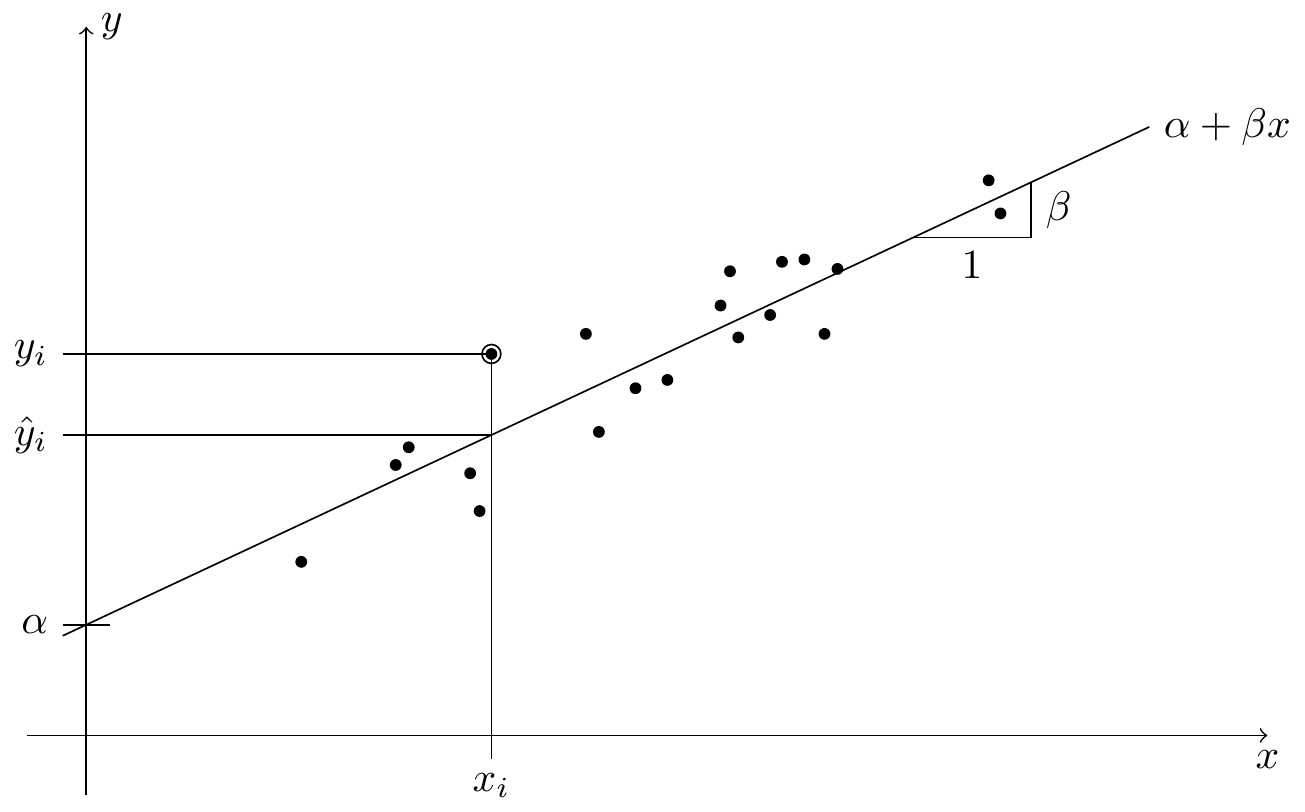
\includegraphics{MATH3714_files/figure-latex/scatter-plot-1} 

}

\caption{An illustration of linear regression. Each of the black circles in the plot stands for one paired sample \((x_i, y_i)\). The regression line \(x \mapsto \alpha + \beta x\), with intercept~\(\alpha\) and slope~\(\beta\), aims to predict the value of~\(y\) using the observed value~\(x\). For the marked sample \((x_i, y_i)\), the predicted \(y\)-value is \(\hat y\).}\label{fig:scatter-plot}
\end{figure}

In this situation, the variable \(x\) is called a \textbf{input}, feature, or
sometimes the explanatory variable or the ``independent variable''.
The variable \(y\) is called \textbf{response} or output, or sometimes the
``dependent variable'', and \(\varepsilon\) is called the \textbf{residual} or error.

Extending the situation of simple linear regression, in this module
we will consider multiple linear regression, where the response~\(y\)
is allowed to depend on several input variables. The corresponding
model is now
\begin{equation*}
  y_i = \alpha + \beta_1 x_{i1} + \cdots + \beta_p x_{ip} + \varepsilon_i
\end{equation*}
for all \(i \in \{1, 2, \ldots, p\}\), where \(n\) is still the number
of observations, and \(p\) is now the number of inputs we observe for
each sample.

Note that for multiple linear regression, we still consider a
single response for each sample, only the number of inputs has been
increased. One way to deal with situations where there is more than
one output would be to fit separate models for each output.

We will discuss multiple linear regression in much detail; our discussion
will be guided by three different aims of linear regression:

\begin{enumerate}
\def\labelenumi{\arabic{enumi}.}
\tightlist
\item
  Prediction: given a not previously observed value \(x\), try to predict
  the corresponding~\(y\).
\item
  In cases were the residuals \(\varepsilon_i\) correspond to unwanted noise,
  the fitted values \(\hat y_i = \alpha + \beta x_i\) can be considered
  to be de-noised versions of the observed values \(y_i\).
\item
  By studying a fitted regression model, sometimes better understanding
  of the data can be achieved. For example, one could ask whether
  all of the \(p\) input variables carry information about the response~\(y\).
\end{enumerate}

We will address these aims by considering different questions, like
how to estimate the coefficients \(\alpha, \beta_1, \ldots, \beta_p\),
how to assess model fit, or how to deal with outliers in the data.

\hypertarget{S00-about}{%
\section*{About MATH3714}\label{S00-about}}
\addcontentsline{toc}{section}{About MATH3714}

This module is \textbf{MATH3714 Linear Regression and Robustness}. The
module manager and lecturer is Dr Jochen Voss, and my email address is
\href{mailto:J.Voss@leeds.ac.uk}{\nolinkurl{J.Voss@leeds.ac.uk}}.

\hypertarget{notes}{%
\subsection*{Notes and videos}\label{notes}}
\addcontentsline{toc}{subsection}{Notes and videos}

The main way I expect you to learn the material for this course is by
reading these notes and by watching the accompanying videos. I will
release two sections of notes each week, for a total of 22 sections.

Reading mathematics is a slow process. Each section roughly
corresponds to one traditional lecture, which would have taken 50
minutes. If you find yourself regularly getting through sections in
much less than an hour, you're probably not reading carefully enough
through each sentence of explanation and each line of mathematics,
including understanding the motivation as well as checking the
accuracy.

It is possible (but not recommended) to learn the material by only
reading the notes and not watching the videos. It is not possible to
learn the material by only watching the videos and not reading the
notes.

Since we will all be relying heavily on these notes, I'm even more
keen than usual to hear about errors mathematical, typographical or
otherwise. Please, please \href{mailto:J.Voss@leeds.ac.uk}{email me} if
think you may have found any.

\hypertarget{lectures}{%
\subsection*{Lectures}\label{lectures}}
\addcontentsline{toc}{subsection}{Lectures}

There will be one online synchronous ``lecture'' session each week, on
Mondays at 2-3pm, with me, run through Microsoft Teams. These will
not be ``lectures'' in the traditional sense of the term, but will be an
opportunity to re-emphasise material you have already learned from
notes and videos, to give extra examples, and to answer common student
questions, with some degree of interactivity.

I will assume you have completed all the work for the previous week by
the time of the lecture, but I will not assume you've started the work
for that week itself.

I am very keen to hear about things you'd like to go through in the
lectures; please \href{mailto:J.Voss@leeds.ac.uk}{email me} with your
suggestions.

\hypertarget{workshops}{%
\subsection*{Workshops and Problem Sheets}\label{workshops}}
\addcontentsline{toc}{subsection}{Workshops and Problem Sheets}

There will be 5 problem sheets, corresponding to workshops in weeks 2,
4, 6, 8 and~10. The main goal of the workshops will be to go over
your answers to the problems sheets.

My recommended approach to problem sheets and workshops is the following:

\begin{itemize}
\tightlist
\item
  Work through the problem sheet before the workshop, spending plenty
  of time on it, and making multiple efforts at questions you get
  stuck on. I recommend spending \emph{at least three hours} on each
  problem sheet, in more than one block. Collaboration is encouraged
  when working through the problems, but I recommend writing up your
  work on your own.
\item
  Take advantage of the workshops to ask for help or clarification on
  questions you weren't able to complete.
\item
  After the workshop, attempt again the questions you were previously stuck on.
\item
  If you're still unable to complete a question after this second
  round of attempts, \emph{then} consult the solutions.
\end{itemize}

\hypertarget{teams}{%
\subsection*{Discussion Board}\label{teams}}
\addcontentsline{toc}{subsection}{Discussion Board}

I have set up \href{https://teams.microsoft.com/l/team/19\%3aopeKURHGjduA41CDtQUkmDjoPalh-zWDGuKhTk9zYq41\%40thread.tacv2/conversations?groupId=bde4675f-2c0d-4efd-9762-748cca83f4c4\&tenantId=bdeaeda8-c81d-45ce-863e-5232a535b7cb}{a Microsoft
Team}
for the course. I propose to use the ``Discussion'' channel there as a
discussion board. This is a good place to post questions about
material from the course, and --- even better! --- to help answer your
colleagues' questions. The idea is that you all as a group should help
each other out. I will visit a couple of times a week to clarify if
everybody is stumped by a question, or if there is disagreement.

\hypertarget{software}{%
\subsection*{Software}\label{software}}
\addcontentsline{toc}{subsection}{Software}

For the module we will use the statistical computing package R. This
program is free software, and you can find the program and
documentation at the \href{https://www.r-project.org/}{R project homepage}.
In particular, R will be used in the (assessed) practial.

My recommendation would be to install the \href{https://www.rstudio.com/}{RStudio
environment}, which includes R, on your own
computer and use this for your work. (Choose the open source
version, ``RStudio Desktop'', on the download page.) Alternatively you
can use RStudio or plain R on the university computers.

\hypertarget{assessments}{%
\subsection*{Assessments}\label{assessments}}
\addcontentsline{toc}{subsection}{Assessments}

Your final mark for the module will be based on a computer practical
(20\%) and a final exam (80\%). For the practical (I believe it will
take place in week 10) you will need to solve some problem using R and
the methods you learned in the course and to present your results in a
short report.

\hypertarget{S01-simple}{%
\section{Simple Linear Regression}\label{S01-simple}}

As a reminder, we consider simple linear regression in this section.
My hope is, that all of you have seen this material before at some
stage, \emph{e.g.}~in school or in some first or second year modules.

In preparation for notation introduced in the next section, we rename
the parameters from \(\alpha\) and \(\beta\) to the new names \(\beta_0\)
for the intercept and \(\beta_1\) for the slope.

\hypertarget{residual-sum-of-squares}{%
\subsection{Residual Sum of Squares}\label{residual-sum-of-squares}}

In simple linear regression, the aim is to find a regression line \(y = \beta_0 + \beta_1 x\), such that the line is ``close'' to given data points
\((x_1, y_1), \ldots, (x_n, y_n) \in\mathbb{R}^2\) for \(i \in \{1, 2, \ldots, n\}\). The ususal way to find \(alpha\) and \(\beta_1\), and thus the regression
line, is by minimising the \textbf{residual sum of squares}:
\begin{equation}
  r(\beta_0, \beta_1)
  = \sum_{i=1}^n \bigl( y_i - (\beta_0 + \beta_1 x_i) \bigr)^2.
  \label{eq:RSS}
\end{equation}
For given \(\beta_0\) and \(\beta_1\), the value \(r(\beta_0, \beta_1)\) measures
how close (in vertical direction) the given data points \((x_i, y_i)\)
are to the regression line \(\beta_0 + \beta_1 x\). By minimising
\(r(\beta_0, \beta_1)\) we find the regression line which is ``closest'' to
the data. The solution of this minimisation problem is usually
expressed in terms of the sample variance \(\mathrm{s}_x\) and the
sample covariance~\(\mathrm{s}_{xy}\).

\begin{definition}
\protect\hypertarget{def:sx}{}\label{def:sx}The \textbf{sample covariance} of \(x_1, \ldots, x_n \in \mathbb{R}\) and
\(y_1, \ldots, y_n\in\mathbb{R}\) is given by
\begin{equation*}
    \mathrm{s}_{xy}
    := \frac{1}{n-1} \sum_{i=1}^n (x_i - \bar x) (y_i - \bar y),
  \end{equation*}
where \(\bar x\) and \(\bar y\) are the sample means.

The \textbf{sample variance} of \(x_1, \ldots, x_n \in \mathbb{R}\) is given by
\begin{equation*}
    \mathrm{s}_{x}^2
    := \mathrm{s}_{xx}
    = \frac{1}{n-1} \sum_{i=1}^n (x_i - \bar x)^2,
  \end{equation*}
where, again, \(\bar x\) is the sample mean of the \(x_i\).
\end{definition}

\begin{lemma}
\protect\hypertarget{lem:simple-LSQ}{}\label{lem:simple-LSQ}Assume that \(\mathrm{s}_x^2 > 0\). Then the function \(r(\beta_0, \beta_1)\)
from~\eqref{eq:RSS} takes its minimum at the point \((\beta_0, \beta_1)\)
given by
\begin{equation*}
    \hat\beta_1 = \frac{\mathrm{s}_{xy}}{\mathrm{s}_x^2},
    \qquad
    \hat\beta_0 = \bar y - \hat \beta_1 \bar x,
  \end{equation*}
where \(\bar x, \bar y\) are the sample means, \(\mathrm{s}_{xy}\) is the
sample covariance and \(\mathrm{s}_x^2\) is the sample variance.
\end{lemma}

\begin{proof}
We could find the minimum of \(r\) by differentiating and setting the
derivatives to zero. Here we follow a different approach which uses
a ``trick'' to simplify the algebra: Let \(\tilde x_i = x_i - \bar x\)
and \(\tilde y_i = y_i - \bar y\) for all \(i \in \{1, \ldots, n\}\).
Then we have
\begin{equation*}
    \sum_{i=1}^n \tilde x_i
    = \sum_{i=1}^n x_i - n \bar x
    = 0
  \end{equation*}
and, similarly, \(\sum_{i=1}^n \tilde y_i = 0\). Using the new
coordinates \(\tilde x_i\) and \(\tilde y_i\) we find
\begin{align*}
    r(\beta_0, \beta_1)
    &= \sum_{i=1}^n \bigl(y_i - \beta_0 - \beta_1 x_i \bigr)^2 \\
    &= \sum_{i=1}^n \bigl( \tilde y_i + \bar y - \beta_0 - \beta_1 \tilde x_i - \beta_1 \bar x \bigr)^2 \\
    &= \sum_{i=1}^n \Bigl( \bigl( \tilde y_i - \beta_1 \tilde x_i \bigr)
    + \bigl( \bar y - \beta_0 - \beta_1 \bar x \bigr) \Bigr)^2 \\
    &= \sum_{i=1}^n \bigl( \tilde y_i - \beta_1 \tilde x_i \bigr)^2
    + 2 \bigl( \bar y - \beta_0 - \beta_1 \bar x \bigr) \sum_{i=1}^n \bigl( \tilde y_i - \beta_1 \tilde x_i \bigr)
    + n \bigl( \bar y - \beta_0 - \beta_1 \bar x \bigr)^2
  \end{align*}
Since \(\sum_{i=1}^n \tilde x_i = \sum_{i=1}^n \tilde y_i = 0\), the
second term on the right-hand side vanishes and we get
\begin{equation}
    r(\beta_0, \beta_1)
    = \sum_{i=1}^n \bigl( \tilde y_i - \beta_1 \tilde x_i \bigr)^2
    + n \bigl( \bar y - \beta_0 - \beta_1 \bar x \bigr)^2.  \label{eq:RSS-rewrite}
  \end{equation}
Both of these terms are positive and we can minimise the second term
(without changing the first term) by setting
\(\beta_0 = \bar y - \beta_1 \bar x\).

To find the value of \(\beta_1\) which minimises the first term on the
right-hand side of~\eqref{eq:RSS-rewrite} we now set the
(one-dimensional) derivative w.r.t.~\(\beta_1\) equal to~\(0\). We get
the condition
\begin{align*}
    0
    &\overset{!}{=} \frac{d}{d\beta_1} \sum_{i=1}^n \bigl( \tilde y_i - \beta_1 \tilde x_i \bigr)^2 \\
    &= \sum_{i=1}^n 2 \bigl( \tilde y_i - \beta_1 \tilde x_i \bigr) \frac{d}{d\beta_1} \bigl( \tilde y_i - \beta_1 \tilde x_i \bigr) \\
    &= - 2 \sum_{i=1}^n \bigl( \tilde y_i - \beta_1 \tilde x_i \bigr) \tilde x_i \\
    &= -2  \sum_{i=1}^n \tilde x_i \tilde y_i + 2 \beta_1 \sum_{i=1}^n \tilde x_i^2.
  \end{align*}
The only solution to this equation is
\begin{align*}
    \beta_1
    &= \frac{\sum_{i=1}^n \tilde x_i \tilde y_i}{\sum_{i=1}^n \tilde x_i^2} \\
    &= \frac{\sum_{i=1}^n (x_i - \bar x) (y_i - \bar y)}%
    {\sum_{i=1}^n (x_i - \bar x)^2} \\
    &= \frac{\frac{1}{n-1}\sum_{i=1}^n (x_i - \bar x) (y_i - \bar y)}%
    {\frac{1}{n-1}\sum_{i=1}^n (x_i - \bar x)^2} \\
    &= \frac{\mathrm{s}_{xy}}{\mathrm{s}_x^2}.
  \end{align*}
Since the second derivative is \(2 \sum_{i=1}^n \tilde x_i^2 \geq 0\),
this is indeed a minimum and the proof is complete.
\end{proof}

\hypertarget{linear-regression-as-a-parameter-estimation-problem}{%
\subsection{Linear Regression as a Parameter Estimation Problem}\label{linear-regression-as-a-parameter-estimation-problem}}

In statistics, any analysis starts by making a statistical model of
the data. This is done by writing random variables which have the
same structure as the data, and which are chosen so that the data
``looks like'' a random sample from these random variables.

To construct a model for the data used in a simple linear regression
problem, we use random variables \(Y_1, \ldots, Y_n\) such that
\begin{equation}
  Y_i
  = \beta_0 + \beta_1 x_i + \varepsilon_i \label{eq:regression}
\end{equation}
for all \(i \in \{1, 2, \ldots, n\}\), where \(\varepsilon_1, \ldots, \varepsilon_n\)
are i.i.d.~random variables with \(\mathbb{E}(\varepsilon_i) = 0\) and
\(\mathop{\mathrm{Var}}(\varepsilon_i) = \sigma^2\).

\begin{itemize}
\tightlist
\item
  Here we assume that the \(x\)-values are fixed and known. The only
  random quantities in the model are \(\varepsilon_i\) and~\(Y_i\). (There are
  more complicated models which also allow for randomness of \(x\), but
  we won't consider such models here.)
\item
  The random variables \(\varepsilon_i\) are called \textbf{residuals} or
  \textbf{errors}. In a scatter plot, the residuals correspond to the
  vertical distance between the samples and the regression line.
  Often one assumes that \(\varepsilon_i \sim \mathcal{N}(0, \sigma^2)\) for all
  \(i \in \{1, 2, \ldots, n\}\).
\item
  The values \(\beta_0\), \(\beta_1\) and \(\sigma^2\) are parameters of
  the model. To fit the model to data, we need to estimate these
  parameters.
\end{itemize}

This model is more complex than the models considered in some
introductory courses to statistics:

\begin{itemize}
\tightlist
\item
  The data consists now of pairs of numbers, instead of just
  single numbers.
\item
  We have
  \begin{equation*}
    \mathbb{E}(Y_i)
    = \mathbb{E}\bigl( \beta_0 + \beta_1 x_i + \varepsilon_i \bigr)
    = \beta_0 + \beta_1 x_i + \mathbb{E}(\varepsilon_i)
    = \beta_0 + \beta_1 x_i.
  \end{equation*}
  Thus, the expectation of \(Y_i\) depends on \(x_i\) and, at least for
  \(\beta_1 \neq 0\), the random variables \(Y_i\) are not identically
  distributed.
\end{itemize}

In this setup, we can consider the estimates \(\hat\beta_0\) and \(\hat\beta_1\)
from the previous subsection as statistcal parameter estimates for the
model parameters \(\beta_0\) and~\(\beta_1\).

In order to fit a linear model we also need to estimate the residual
variance~\(\sigma^2\). This can be done using the estimator
\begin{equation}
  \hat\sigma^2
  = \frac{1}{n-2} \sum_{i=1}^n \hat\varepsilon_i^2
  = \frac{1}{n-2} \sum_{i=1}^n (y_i - \hat\beta_0 - \hat\beta_1 x_i)^2.
  \label{eq:reg-sigma-est}
\end{equation}
To understand the form of this estimator, we have to remember that
\(\sigma^2\) is the variance of the \(\varepsilon_i\). Thus, using the standard
estimator for the variance, we could estimate \(\sigma^2\) as
\begin{equation}
  \sigma^2
  \approx \frac{1}{n-1} \sum_{i=1}^n \bigl(\varepsilon_i - \bar\varepsilon\bigr)^2
  \approx \frac{1}{n-1} \sum_{i=1}^n \bigl(\hat\varepsilon_i - \overline{\hat\varepsilon}\bigr)^2,
  \label{eq:resid-var-est}
\end{equation}

where \(\bar\varepsilon\) and \(\overline{\hat\varepsilon}\) are the averages of the
\(\varepsilon_i\) and the \(\hat\varepsilon_i\), respectively. One can show that
\(\overline{\hat\varepsilon} = 0\). The estimates of \(\beta_0\) and \(\beta_1\) are
sensitive to fluctuations in the data, with the effect that the
estimated regression line is, on average, slightly closer to the data
points than the true regression line would be. This causes the sample
variance of the \(\hat\varepsilon_i\), on average, to be slightly smaller than
the true residual variance \(\sigma^2\) and the thus the
estimator~\eqref{eq:resid-var-est} is slightly biased. A more
detailed analysis reveals that an unbiased estimator can be obtained
if one replaces the pre-factor \(1/(n-1)\) in equation~\eqref{eq:resid-var-est}
with \(1/(n-2)\). This leads to the estimator~\eqref{eq:reg-sigma-est}.

The main advantage gained by considering a statistical model is, that
we now can consider how close the estimators \(\hat\beta_0\), \(\hat\beta_1\)
and \(\hat\sigma^2\) are to the true values. Results one can obtain
include the following:

\begin{itemize}
\item
  The estimators \(\hat\beta_0\), \(\hat\beta_1\) and \(\hat\sigma^2\)
  are unbiased: This means that when we plug in random data
  \((x_i, Y_i)\) from the model~\eqref{eq:regression}, on
  average we get the correc answer: \(\mathbb{E}(\hat\beta_0) = \beta_0\),
  \(\mathbb{E}(\hat\beta_1) = \beta_1\), \(\mathbb{E}(\hat\sigma^2) = \sigma^2\).
\item
  One can ask about the average distance between the estimated
  parameters \(\hat\beta_0\), \(\hat\beta_1\) and \(\hat\sigma^2\)
  and the (unknown) true values \(\beta_0\), \(\beta_1\) and \(\sigma^2\).
  One measure for these distances is the root mean squared error
  of the estimators.
\item
  One can consider confidence intervals for the parameters
  \(\beta_0\), \(\beta_1\) and \(\sigma^2\).
\item
  One can consider statistical hypothesis tests to answer
  yes/no questions about the parameters. For example, one might ask
  whether the data could have come from the model with \(\beta_0=0\).
\item
  One can consider whether the data is compatible with the model
  at all, irrespective of parameter values. If there is a non-linear
  relationship between \(x\) and \(y\), the model~\eqref{eq:regression}
  will no longer be appropriate.
\end{itemize}

We will consider most of these questions over the course of the
module.

\hypertarget{sec:simple-mat}{%
\subsection{Matrix Notation}\label{sec:simple-mat}}

To conclude this section, we will rewrite the results of this section
in a form which we will extensively use for multiple linear regression
in the rest of this module. The idea here is to arrange all quantities
in the problem as matrices and vectors in order to simplify notation.
We write
\begin{equation*}
  X = \begin{pmatrix}
    1 & x_1\\ 1 & x_2\\\vdots & \vdots\\1 & x_n
  \end{pmatrix}
  \in \mathbb{R}^{n\times 2},
  \qquad
  y = \begin{pmatrix}
    y_1 \\ y_2 \\ \vdots \\ y_n
  \end{pmatrix}
  \in \mathbb{R}^n,
  \qquad
  \varepsilon= \begin{pmatrix}
    \varepsilon_1 \\ \varepsilon_2 \\ \vdots \\ \varepsilon_n
  \end{pmatrix}
  \in \mathbb{R}^n,
  \qquad
  \beta = \begin{pmatrix}
    \beta_0 \\
    \beta_1
  \end{pmatrix}
  \in\mathbb{R}^2
\end{equation*}
Using this notation, we can rewrite the \(n\) equations \(y_i = \beta_0 + x_i \beta_1 + \varepsilon_i\) for \(i \in \{1, \ldots, n\}\) as one
vector-valued equation in~\(\mathbb{R}^n\): we get
\begin{equation*}
  y = X\beta + \varepsilon,
\end{equation*}
and we want to ``solve'' this vector-valued equation for~\(\beta\).
The sum of squares can now be written as
\begin{equation*}
  r(\beta)
  = \sum_{i=1}^n \varepsilon_i^2
  = \varepsilon^\top \varepsilon
  = (y - X\beta)^\top (y - X\beta)
  = y^\top y - 2\beta^\top X^\top y + \beta^\top X^\top X \beta.
\end{equation*}
In the next section we will see that the minimum of \(r\) is attained
for
\begin{equation*}
  \hat\beta
  = (X X^\top)^{-1} X^\top y
\end{equation*}
and one can check that the components of this vector \(\hat\beta = (\hat\beta_0, \hat\beta_1)\) coincide with the estimates we obtained above.

\textbf{Summary}

\begin{itemize}
\tightlist
\item
  simple linear regression is the case where there is only one input
\item
  a regression line is fitted by minimising the residual sum of squares
\item
  linear regression is a statistical parameter estimation problem
\item
  the problem can be conveniently written in matrix/vector notation
\end{itemize}

\hypertarget{S02-multiple}{%
\section{Least Squares Estimates}\label{S02-multiple}}

\hypertarget{data-and-models}{%
\subsection{Data and Models}\label{data-and-models}}

For multiple linear regression we assume that there are \(p\) inputs and
one output. If we have a sample of \(n\) obervations, we have \(np\)
inputs and one output in total. Here we denote the \(i\)th observation
of the \(j\)th input by \(x_{ij}\) and the corresponding output by~\(y_j\).

As an example, we consider the \texttt{mtcars} dataset built into R. This is
a small dataset, which contains information about 32 automobiles
(1973--74 models). The table lists fuel consumption \texttt{mpg}, gross horsepower \texttt{hp},
and 9 other aspects of these cars. Here we consider \texttt{mpg} to be the output,
and the other listed aspects to be inputs. Type \texttt{help(mtcars)} in R to learn
more about this dataset:

\begin{Shaded}
\begin{Highlighting}[]
\NormalTok{mtcars}
\end{Highlighting}
\end{Shaded}

\begin{verbatim}
##                      mpg cyl  disp  hp drat    wt  qsec vs am gear carb
## Mazda RX4           21.0   6 160.0 110 3.90 2.620 16.46  0  1    4    4
## Mazda RX4 Wag       21.0   6 160.0 110 3.90 2.875 17.02  0  1    4    4
## Datsun 710          22.8   4 108.0  93 3.85 2.320 18.61  1  1    4    1
## Hornet 4 Drive      21.4   6 258.0 110 3.08 3.215 19.44  1  0    3    1
## Hornet Sportabout   18.7   8 360.0 175 3.15 3.440 17.02  0  0    3    2
## Valiant             18.1   6 225.0 105 2.76 3.460 20.22  1  0    3    1
## Duster 360          14.3   8 360.0 245 3.21 3.570 15.84  0  0    3    4
## Merc 240D           24.4   4 146.7  62 3.69 3.190 20.00  1  0    4    2
## Merc 230            22.8   4 140.8  95 3.92 3.150 22.90  1  0    4    2
## Merc 280            19.2   6 167.6 123 3.92 3.440 18.30  1  0    4    4
## Merc 280C           17.8   6 167.6 123 3.92 3.440 18.90  1  0    4    4
## Merc 450SE          16.4   8 275.8 180 3.07 4.070 17.40  0  0    3    3
## Merc 450SL          17.3   8 275.8 180 3.07 3.730 17.60  0  0    3    3
## Merc 450SLC         15.2   8 275.8 180 3.07 3.780 18.00  0  0    3    3
## Cadillac Fleetwood  10.4   8 472.0 205 2.93 5.250 17.98  0  0    3    4
## Lincoln Continental 10.4   8 460.0 215 3.00 5.424 17.82  0  0    3    4
## Chrysler Imperial   14.7   8 440.0 230 3.23 5.345 17.42  0  0    3    4
## Fiat 128            32.4   4  78.7  66 4.08 2.200 19.47  1  1    4    1
## Honda Civic         30.4   4  75.7  52 4.93 1.615 18.52  1  1    4    2
## Toyota Corolla      33.9   4  71.1  65 4.22 1.835 19.90  1  1    4    1
## Toyota Corona       21.5   4 120.1  97 3.70 2.465 20.01  1  0    3    1
## Dodge Challenger    15.5   8 318.0 150 2.76 3.520 16.87  0  0    3    2
## AMC Javelin         15.2   8 304.0 150 3.15 3.435 17.30  0  0    3    2
## Camaro Z28          13.3   8 350.0 245 3.73 3.840 15.41  0  0    3    4
## Pontiac Firebird    19.2   8 400.0 175 3.08 3.845 17.05  0  0    3    2
## Fiat X1-9           27.3   4  79.0  66 4.08 1.935 18.90  1  1    4    1
## Porsche 914-2       26.0   4 120.3  91 4.43 2.140 16.70  0  1    5    2
## Lotus Europa        30.4   4  95.1 113 3.77 1.513 16.90  1  1    5    2
## Ford Pantera L      15.8   8 351.0 264 4.22 3.170 14.50  0  1    5    4
## Ferrari Dino        19.7   6 145.0 175 3.62 2.770 15.50  0  1    5    6
## Maserati Bora       15.0   8 301.0 335 3.54 3.570 14.60  0  1    5    8
## Volvo 142E          21.4   4 121.0 109 4.11 2.780 18.60  1  1    4    2
\end{verbatim}

For this dataset we have \(n = 32\) (number of cars), and \(p = 10\) (number
of attributes, excluding \texttt{mpg}). The values \(y_1, \ldots, y_{32}\) are listed
in the first column of the table, the values \(x_{i,1}\) for \(i \in \{1, \ldots, 32\}\) are shown in the second column, and the values \(x_{i,10}\) are shown in
the last column.

In this data set it is easy to make scatter plots which show how a single
input affects the output. For example, we can show how the engine power
affects fuel consumption:

\begin{Shaded}
\begin{Highlighting}[]
\FunctionTok{plot}\NormalTok{(mtcars}\SpecialCharTok{$}\NormalTok{hp, mtcars}\SpecialCharTok{$}\NormalTok{mpg,}
     \AttributeTok{xlab =} \StringTok{"power [hp]"}\NormalTok{, }\AttributeTok{ylab =} \StringTok{"fuel consumption [mpg]"}\NormalTok{)}
\end{Highlighting}
\end{Shaded}

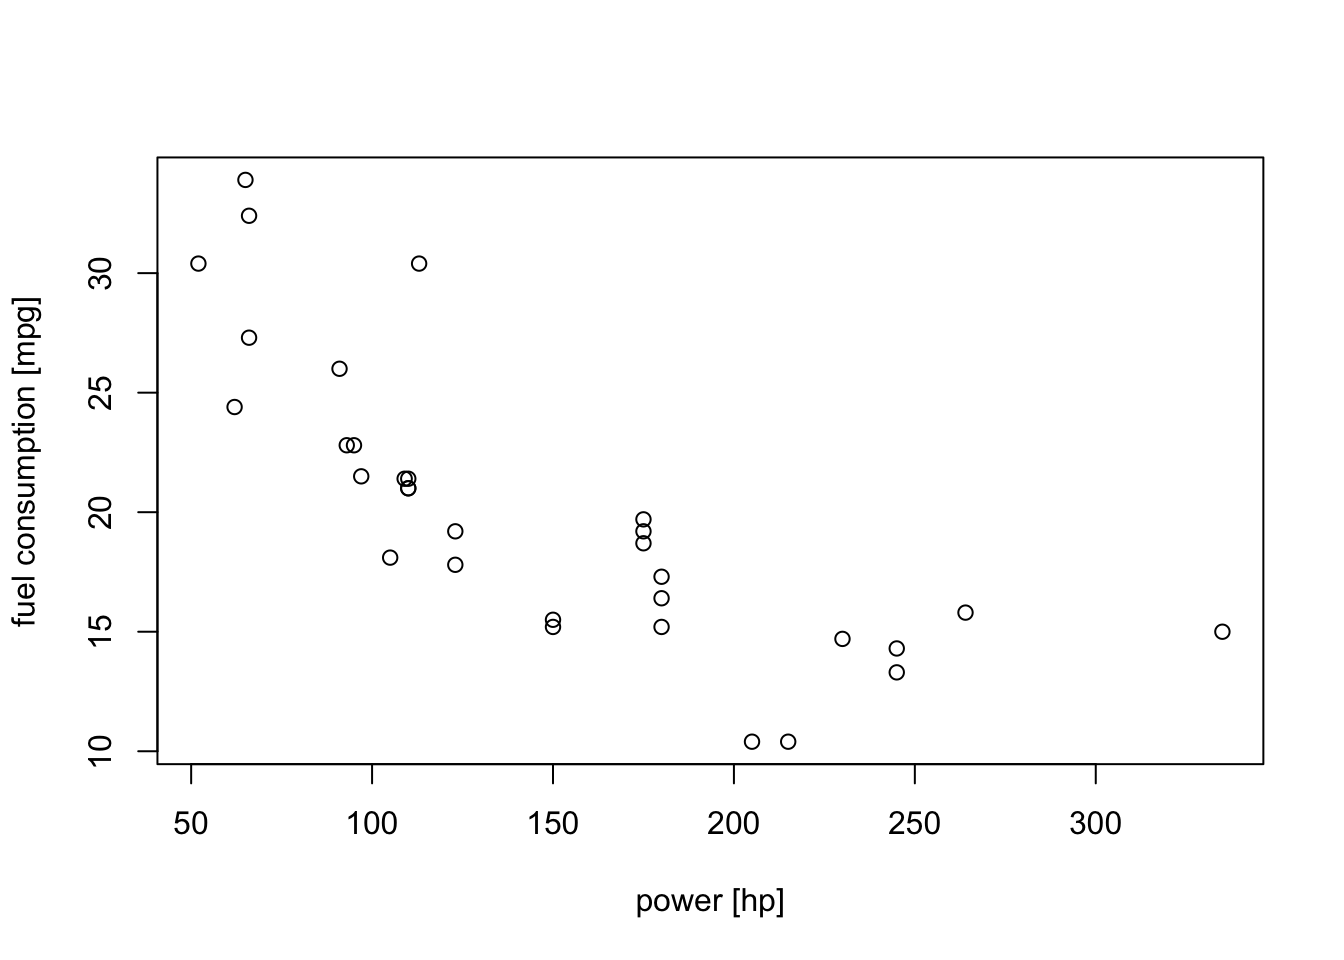
\includegraphics{MATH3714_files/figure-latex/unnamed-chunk-2-1.pdf}

We can see that cars with stronger engines tend to use more fuel
(\emph{i.e.}~a gallon of fuel lasts for fewer miles; the curve goes down),
but leaving out the other inputs omits a lot of information. It is
not easy to make a plot which takes all inputs into account. Is is
also not immediately obvious which of the variables are most
important.

In linear regression, we assume that the output depends on the
inputs in a linear (or more precisely, \emph{affine}) way. We write
this as
\begin{equation}
  y_i
  = \beta_0 + \beta_1 x_{i,1} + \cdots + \beta_p x_{i,p} + \varepsilon_i \label{eq:lmdata}
\end{equation}
where the residuals~\(\varepsilon_i\) are assumed to be ``small''.

The parameters \(\beta_j\) can be interpreted as the expected change in
the response \(y\) per unit change in \(x_j\) when all other regressor
variables are held fixed. For this reason the parameters \(\beta_j\)
(for \(j=1, \ldots, p\)) are sometimes called \emph{partial} regression
coefficients.

This model describes a hyperplane in the \((p+1)\)-dimensional space of
the inputs \(x_j\) and the output~\(y\). The hyperplane is easily
visualized when \(p=1\) (as a line in~\(\mathbb{R}^2\)), and visualisation can be
attempted for \(p=2\) (as a plane in \(\mathbb{R}^3\)) but is very hard for \(p>2\).

We defer making a proper statistical model for multiple linear regression
until the next section.

\hypertarget{the-normal-equations}{%
\subsection{The Normal Equations}\label{the-normal-equations}}

Similar to what we did in Section~\ref{sec:simple-mat}, we rewrite
the model using matrix notation. We define the vectors
\begin{equation*}
  y = \begin{pmatrix}
    y_1 \\ y_2 \\ \vdots \\ y_n
  \end{pmatrix}
  \in \mathbb{R}^n,
  \qquad
  \varepsilon= \begin{pmatrix}
    \varepsilon_1 \\ \varepsilon_2 \\ \vdots \\ \varepsilon_n
  \end{pmatrix}
  \in \mathbb{R}^n,
  \qquad
  \beta = \begin{pmatrix}
    \beta_0 \\
    \beta_1 \\
    \vdots \\
    \beta_p
  \end{pmatrix}
  \in\mathbb{R}^{1+p}
\end{equation*}
as well as the matrix
\begin{equation*}
  X = \begin{pmatrix}
    1 & x_{1,1} & \cdots & x_{1,p} \\
    1 & x_{2,1} & \cdots & x_{2,p} \\
    \vdots & \vdots & & \vdots \\
    1 & x_{n,1} & \cdots & x_{n,p} \\
  \end{pmatrix}
  \in \mathbb{R}^{n\times (1+p)}.
\end{equation*}
The matrix \(X\) is often called the \textbf{design matrix}.

Using this notation, the model~\eqref{eq:lmdata} can be written
as
\begin{equation}
  y = X \beta + \varepsilon,  \label{eq:lmmodel}
\end{equation}
where again \(X\beta\) is a matrix-vector multiplication which ``hides''
the sums in equation~\eqref{eq:lmdata}, and \eqref{eq:lmmodel}
is an equation of vectors of size~\(n\), which combines the \(n\)
individual equations from \eqref{eq:lmdata} for the different
values of~\(i\).

To simplify notation, we index the columns of \(X\) by \(0, 1, \ldots, p\) (instead of the more conventional \(1, \ldots, p+1\)), so that we
can for example write
\begin{equation*}
  (X \beta)_i
  = \sum_{j=0}^p x_{i,j} \beta_j
  = \beta_0 + \sum_{j=1}^p x_{i,j} \beta_j.
\end{equation*}

As before, we find the regression coefficients by minimising
the residual sum of squares:
\begin{align*}
  r(\beta)
  &= \sum_{i=1}^n \varepsilon_i^2 \\
  &= \sum_{i=1}^n \bigl( y_i - (\beta_0 + \beta_1 x_{i,1} + \cdots + \beta_p x_{i,p}) \bigr)^2.
\end{align*}
In practice, this notation turns out to be cumbersome, and we will
use matrix notation in the following proof.

\begin{lemma}
\protect\hypertarget{lem:multiple-LSQ}{}\label{lem:multiple-LSQ}Assume that the matrix \(X^\top X \in \mathbb{R}^{(1+p) \times (1+p)}\) is
invertible. Then the function \(r(\beta)\) takes its minimum at the
vector \(\hat\beta\in\mathbb{R}^{p+1}\) given by
\begin{equation*}
  \hat\beta
  = (X^\top X)^{-1} X^\top y.
\end{equation*}
\end{lemma}

\begin{proof}
Using the vector equation \(\varepsilon= y - X \beta\), we can also write the
residual sum of squares as
\begin{align*}
    r(\beta)
    &= \sum_{i=1}^n \varepsilon_i^2 \\
    &= \varepsilon^\top \varepsilon\\
    &= (y - X \beta)^\top (y - X \beta) \\
    &= y^\top y - y^\top X\beta - (X\beta)^\top y + (X\beta)^\top (X\beta).
  \end{align*}
Using the linear algebra rules from Appendix~\ref{matrix-rules} we find
that \(y^\top X\beta = (X\beta)^\top y = \beta^\top X^\top y\)
and \((X\beta)^\top (X\beta) = \beta^\top X^\top X \beta\). Thus we get
\begin{equation*}
    r(\beta)
    = y^\top y - 2\beta^\top X^\top y + \beta^\top X^\top X \beta.
  \end{equation*}
Note that in this eqation \(X\) is a matrix, \(y\) and \(\beta\) are vectors,
and \(r(\beta)\) is a number.

To find the minimum of this function, we set all partial derivatives
\(\frac{\partial}{\partial \beta_i} r(\beta)\) equal to~\(0\). Going through the terms in
the formula for \(r(\beta)\) we find: (1) \(y^\top y\) does not depend on \(\beta\),
so we have \(\frac{\partial}{\partial \beta_i} y^\top y = 0\) for all \(i\), (2) we have
\begin{equation*}
    \frac{\partial}{\partial \beta_i} \beta^\top X^\top y
    = \frac{\partial}{\partial \beta_i} \sum_{j=1}^{p+1} \beta_j (X^\top y)_j
    = (X^\top y)_i
  \end{equation*}
and (3) finally
\begin{equation*}
    \frac{\partial}{\partial \beta_i} \beta^\top X^\top X \beta
    = \frac{\partial}{\partial \beta_i} \sum_{j,k=1}^{p+1} \beta_j (X^\top X)_{j,k} \beta_k
    = 2 \sum_{k=1}^{p+1} (X^\top X)_{i,k} \beta_k
    = 2 \bigl( (X^\top X) \beta \bigr)_i.
  \end{equation*}
(Some care is needed, when checking that the middle equality sign in
the previous equation is correct.)
Combining these derivatives, we find
\begin{equation}
    \frac{\partial}{\partial \beta_i} r(\beta)
    = 0 - 2 (X^\top y)_i + 2 \bigl( (X^\top X)_{i,k} \beta \bigr)_i
                           \label{eq:normal-first}
  \end{equation}
for all \(i \in \{0, 1, \ldots, p\}\). At a local minimum of \(r\),
all of these partial derivatives must be zero and using a vector
equation we find that a necessary condition for a minimum is
\begin{equation}
    X^\top X \beta = X^\top y.  \label{eq:normal-equations}
  \end{equation}
Since we assumed that \(X^\top X\) is invertible, there is exactly
one vector \(beta\) which solves \eqref{eq:normal-equations}. This
vector is given by
\begin{equation*}
    \hat\beta
    := (X^\top X)^{-1} X^\top y.
  \end{equation*}

As for one-dimensional minimisation, there is a condition on the
second derivatives which must be checked to see which local extrema
are local minima. Here we are only going to sketch this argument: A
sufficient condition for \(\hat\beta\) to be a minimum is for the
second derivative matrix (\href{https://en.wikipedia.org/wiki/Hessian_matrix}{the Hessian
matrix})
to be positive definite (see appendix \ref{positive-definite}).
Using equation~\eqref{eq:normal-first} we find
\begin{equation*}
    \frac{\partial}{\partial\beta_i \partial\beta_j} r(\beta)
    = 2 (X^\top X)_{i,j}
  \end{equation*}
And thus the Hessian matrix is \(H = 2 X^\top X\). Using results from
linear algebra, one can show that this matrix is indeed positive
definite and thus \(\hat\beta\) is the unique minimum of~\(r\).
\end{proof}

Equation~\eqref{eq:normal-equations} gives a system of \(p+1\) linear
equations with \(p+1\) unknowns. This system of linear equations,
\(X^\top X \beta = X^\top y\) is called the \textbf{normal equations}.
If \(X^\top X\) is invertible, as assumed in the lemma, this
system of equations has \(\hat\beta\) as its unique solution.
Otherwise, there may be more than one \(\beta\) which leads to the
same value \(r(\beta)\) and the minimum will no longer be unique.
This happens for example, if two of the inputs are identical to
each other (or, more generally, one input is linearly dependent
on one or more other inputs).

The condition that \(X^\top X\) must be invertible in multiple linear
regression corresponds to the condition \(\mathrm{s}_x^2 > 0\) from
lemma~\ref{lem:simple-LSQ} for simple linear regression.

The value \(\hat\beta\) found in the lemma is called the \textbf{least squares
estimator} for \(\beta\), or sometimes the ordinary least squares (OLS)
estimator.

\hypertarget{fitted-values}{%
\subsection{Fitted Values}\label{fitted-values}}

Let us again consider our model
\begin{equation*}
  y = X \beta + \varepsilon,
\end{equation*}
using the matrix notation introduced above. Here we can think of
\(X\beta\) as the \textbf{true values}, while \(\varepsilon\) are the errors. The
design matrix \(X\) (containing the inputs) and the response \(y\) are
known to us, while the true coefficients \(\beta\) and the errors \(\varepsilon\)
are unknown. Solving for \(\varepsilon\) we find that the errors satisfy
\begin{equation*}
  \varepsilon= y - X\beta.
\end{equation*}

Using the least squares estimate \(\hat\beta\) we can estimate the true
values as
\begin{equation*}
  \hat y = X \hat\beta.
\end{equation*}
These estimates are called the \textbf{fitted values}. Using the
definition of \(\hat\beta\) we get
\begin{equation*}
  \hat y
  = X (X^\top X)^{-1} X^\top y
  =: Hy.
\end{equation*}
The matrix \(H = X (X^\top X)^{-1} X^\top\) is commonly called the \textbf{hat
matrix} (because it ``puts the hat on \(y\)'').

Finally, we can estimate the errors using the residuals
\begin{equation*}
  \hat\varepsilon
  = y - X \hat\beta
  = y - \hat y
  = y - H y
  = (I - H) y,
\end{equation*}
where \(I\) is the \((p+1)\times (p+1)\) identity matrix.

\hypertarget{example}{%
\subsection{Example}\label{example}}

To conclude this section, we demonstrate how these methods can be used
in R. For this we consider the \texttt{mtcars} example from the beginning of
the section again. I will first show how to do the analysis ``by hand'',
and later show how the same result can be obtained using R's built-in functions.

We first split \texttt{mtcars} into the respons column \texttt{y} (the first column)
and the design matrix \texttt{X} (a column of ones, followed by columns 2 to 11
of \texttt{mtcars}):

\begin{Shaded}
\begin{Highlighting}[]
\NormalTok{y }\OtherTok{\textless{}{-}}\NormalTok{ mtcars[, }\DecValTok{1}\NormalTok{]}
\NormalTok{X }\OtherTok{\textless{}{-}} \FunctionTok{cbind}\NormalTok{(}\DecValTok{1}\NormalTok{, }\FunctionTok{data.matrix}\NormalTok{(mtcars[, }\DecValTok{2}\SpecialCharTok{:}\DecValTok{11}\NormalTok{]))}
\end{Highlighting}
\end{Shaded}

Next we compute \(X^\top X\) and solve the normal equations. Often it is
faster, easier, and has lower numerical errors to solve the normal equations
rather than inverting the matrix \(X^\top X\).

\begin{Shaded}
\begin{Highlighting}[]
\NormalTok{XtX }\OtherTok{\textless{}{-}} \FunctionTok{t}\NormalTok{(X) }\SpecialCharTok{\%*\%}\NormalTok{ X}
\NormalTok{beta.hat }\OtherTok{\textless{}{-}} \FunctionTok{solve}\NormalTok{(XtX, }\FunctionTok{t}\NormalTok{(X) }\SpecialCharTok{\%*\%}\NormalTok{ y)}
\NormalTok{beta.hat}
\end{Highlighting}
\end{Shaded}

\begin{verbatim}
##             [,1]
##      12.30337416
## cyl  -0.11144048
## disp  0.01333524
## hp   -0.02148212
## drat  0.78711097
## wt   -3.71530393
## qsec  0.82104075
## vs    0.31776281
## am    2.52022689
## gear  0.65541302
## carb -0.19941925
\end{verbatim}

Without further checks it is hard to know whether the result is correct, or
whether we made a mistake somewhere along the lines. One good sign is that
we argued earlier that higher \texttt{hp} should lead to lower \texttt{mpg}, and indeed the
corresponding coefficient \texttt{-0.02148212} is negative.

Finally, compute the fitted values and generate a plot of fitted values
against responses. If everything worked, we would expect the points in this
plot to be close to the diagonal.

\begin{Shaded}
\begin{Highlighting}[]
\NormalTok{y.hat }\OtherTok{\textless{}{-}}\NormalTok{ X }\SpecialCharTok{\%*\%}\NormalTok{ beta.hat}
\FunctionTok{plot}\NormalTok{(y, y.hat, }\AttributeTok{xlab =} \StringTok{"responses"}\NormalTok{, }\AttributeTok{ylab =} \StringTok{"fitted values"}\NormalTok{)}
\FunctionTok{abline}\NormalTok{(}\AttributeTok{a =} \DecValTok{0}\NormalTok{, }\AttributeTok{b =} \DecValTok{1}\NormalTok{) }\CommentTok{\# plot the diagonal}
\end{Highlighting}
\end{Shaded}

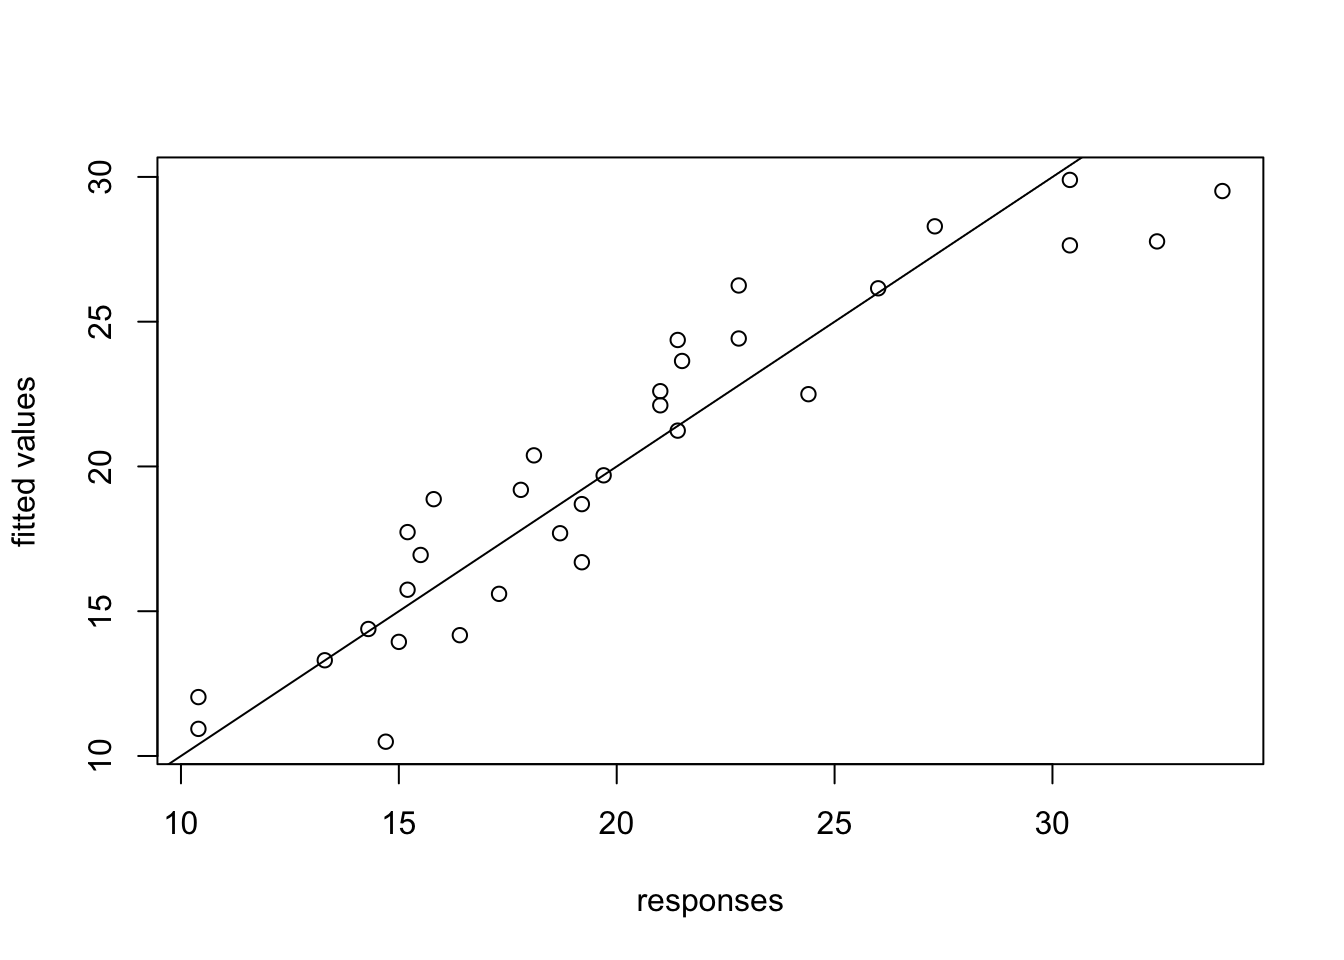
\includegraphics{MATH3714_files/figure-latex/unnamed-chunk-5-1.pdf}

For comparison we now re-do the analysis using built-in R commands.
In the \texttt{lm()} command below, we use \texttt{data=mtcars} to tell R where the
data is stored, and the formula \texttt{mpg\ \textasciitilde{}\ .} states that we want to
model \texttt{mpg} as a function of all other variable (this is the meaning of \texttt{.}).

\begin{Shaded}
\begin{Highlighting}[]
\NormalTok{m }\OtherTok{\textless{}{-}} \FunctionTok{lm}\NormalTok{(mpg }\SpecialCharTok{\textasciitilde{}}\NormalTok{ ., }\AttributeTok{data =}\NormalTok{ mtcars) }\CommentTok{\# fit a linear model}
\FunctionTok{coef}\NormalTok{(m) }\CommentTok{\# get the estimated coefficients}
\end{Highlighting}
\end{Shaded}

\begin{verbatim}
## (Intercept)         cyl        disp          hp        drat          wt 
## 12.30337416 -0.11144048  0.01333524 -0.02148212  0.78711097 -3.71530393 
##        qsec          vs          am        gear        carb 
##  0.82104075  0.31776281  2.52022689  0.65541302 -0.19941925
\end{verbatim}

Comparing these coefficients to the vector \texttt{beta.hat} from above shows
that we got the same result using both methods. The fitted values
can be computed using \texttt{fitted.values(m)}. Here we just check that we get
the same result as above:

\begin{Shaded}
\begin{Highlighting}[]
\FunctionTok{max}\NormalTok{(}\FunctionTok{abs}\NormalTok{(}\FunctionTok{fitted.values}\NormalTok{(m) }\SpecialCharTok{{-}}\NormalTok{ y.hat))}
\end{Highlighting}
\end{Shaded}

\begin{verbatim}
## [1] 5.329071e-13
\end{verbatim}

This results \texttt{5.329071e-13} stands for the number \(5.329071 \cdot 10^{-13}\),
which is extremely small. The difference between our results and R's result
is caused by rounding errors.

\textbf{Summary}

\begin{itemize}
\tightlist
\item
  multiple linear regression allows for more than one input
  but still has only one output
\item
  the least squared estimate for the coefficients is found
  by minimising the residual sum of squares
\item
  the estimate can be computed as the solution to the normal equations
\item
  the hat matrix transforms responses into fitted values
\end{itemize}

\hypertarget{I01-lm}{%
\section*{Interlude: Linear Regression in R}\label{I01-lm}}
\addcontentsline{toc}{section}{Interlude: Linear Regression in R}

\hypertarget{lm-fitting}{%
\subsection*{Specifying a Model}\label{lm-fitting}}
\addcontentsline{toc}{subsection}{Specifying a Model}

The function \texttt{lm()} is used to fit a linear model in~R. There are different
ways to specify the form of the model and the data to be used for fitting the
model.

\begin{itemize}
\item
  The most basic way to call \texttt{lm()} is the case where the explanatory
  variables and the response variable are stored as separate vectors.
  Assuming, for example, that the explanatory variables are \texttt{x1}, \texttt{x2}, \texttt{x3}
  and that the response variable is~\texttt{y} in~R, we can tell R to fit the
  linear model \(y = \beta_0 + \beta_1 x_1 + \beta_2 x_2 + \beta_3 x_3 + \varepsilon\)
  by using the following command:

\begin{Shaded}
\begin{Highlighting}[]
  \FunctionTok{lm}\NormalTok{(y }\SpecialCharTok{\textasciitilde{}}\NormalTok{ x1 }\SpecialCharTok{+}\NormalTok{ x2 }\SpecialCharTok{+}\NormalTok{ x3)}
\end{Highlighting}
\end{Shaded}

  Note that R automatically added the intercept term \(\beta_0\) to this
  model. If we want to fit a model without an intercept,
  \emph{i.e.} the model
  \(y = \beta_1 x_1 + \beta_2 x_2 + \beta_3 x_3 + \varepsilon\), we have to add
  \texttt{0\ +} in front of the explanatory variables:

\begin{Shaded}
\begin{Highlighting}[]
    \FunctionTok{lm}\NormalTok{(y }\SpecialCharTok{\textasciitilde{}} \DecValTok{0} \SpecialCharTok{+}\NormalTok{ x1 }\SpecialCharTok{+}\NormalTok{ x2 }\SpecialCharTok{+}\NormalTok{ x3)}
\end{Highlighting}
\end{Shaded}

  The general form of a model specification is the response variable,
  followed by \texttt{\textasciitilde{}}, followed by a plus-separated list of explanatory
  variables. For this form of calling \texttt{lm()}, the variables \texttt{y},
  \texttt{x1}, \texttt{x2}, and \texttt{x3} in the examples above must be already defined before
  \texttt{lm()} is called. It may be a good idea to double-check that the variables
  have the correct values before trying to call~\texttt{lm()}.
\item
  Both for the response and for explanatory variables we can
  specify arbitrary R expressions to compute the numeric values to be
  used. For example, to fit the model
  \(\log(y) = \beta_0 + \beta_1 x_1 + \beta_2 x_2 + \varepsilon\) (assuming
  that all \(y_i\) are positive) we can use the following command:

\begin{Shaded}
\begin{Highlighting}[]
  \FunctionTok{lm}\NormalTok{(}\FunctionTok{log}\NormalTok{(y) }\SpecialCharTok{\textasciitilde{}}\NormalTok{ x1 }\SpecialCharTok{+}\NormalTok{ x2)}
\end{Highlighting}
\end{Shaded}

  Some care is needed, because \texttt{+}, \texttt{*} and \texttt{\^{}} have a
  special meaning inside the first argument of \texttt{lm()}; any time
  we want to compute a variable for \texttt{lm()} using these
  operations, we need to surround the corresponding expression with
  \texttt{I()}, to tell R that \texttt{+}, \texttt{*} or \texttt{\^{}} should
  have their usual, arithmetic meaning. For example, to fit a model
  of the form \(y \sim \beta_0 + \beta_1 x + \beta_2 x^2 + \varepsilon\), we
  can use the following R command:

\begin{Shaded}
\begin{Highlighting}[]
  \FunctionTok{lm}\NormalTok{(y }\SpecialCharTok{\textasciitilde{}}\NormalTok{ x }\SpecialCharTok{+} \FunctionTok{I}\NormalTok{(x}\SpecialCharTok{\^{}}\DecValTok{2}\NormalTok{))}
\end{Highlighting}
\end{Shaded}

  Here, the use of \texttt{I()} tells R that \texttt{x\^{}2} is to be
  interpreted as the vector \((x_1^2, \ldots, x_n^2)\). Similarly, we
  can fit a model of the form
  \(y = \beta_0 + \beta_1 (x_1 + x_2) + \varepsilon\):

\begin{Shaded}
\begin{Highlighting}[]
  \FunctionTok{lm}\NormalTok{(y }\SpecialCharTok{\textasciitilde{}} \FunctionTok{I}\NormalTok{(x1}\SpecialCharTok{+}\NormalTok{x2))}
\end{Highlighting}
\end{Shaded}

  Here, the use of \texttt{I()} tells R that \texttt{x1+x2} indicates the
  vector \((x_{1,1}+x_{2,1}, \ldots, x_{1,n}+x_{2,n})\) instead of two
  separate explanatory variables.

  Details about how to specify models in calls to \texttt{lm()} can be found by
  using the \href{https://rdrr.io/r/stats/formula.html}{command \texttt{help(formula)}}
  in~R.
\item
  If the response and the explanatory variables are stored in the
  columns of a data frame, we can use the \texttt{data=...} argument to \texttt{lm()} to
  specify this data frame and then just use the column names to specify the
  regression model. For example, the
  \href{https://rdrr.io/r/datasets/stackloss.html}{\texttt{stackloss} data set}
  built into R consists of a data frame with columns \texttt{Air.Flow},
  \texttt{Water.Temp}, \texttt{Acid.Conc.}, \texttt{stack.loss}. To predict
  \texttt{stackloss\$stack.loss} from \texttt{stackloss\$Air.Flow} we can write

\begin{Shaded}
\begin{Highlighting}[]
  \FunctionTok{lm}\NormalTok{(stack.loss }\SpecialCharTok{\textasciitilde{}}\NormalTok{ Air.Flow, }\AttributeTok{data=}\NormalTok{stackloss)}
\end{Highlighting}
\end{Shaded}

  As a special case, a single dot ``\texttt{.}'' can be used in place of
  the explanatory variables in the model to indicate that all columns
  except for the given response should be used. Thus, the following
  two commands are equivalent:

\begin{Shaded}
\begin{Highlighting}[]
  \FunctionTok{lm}\NormalTok{(stack.loss }\SpecialCharTok{\textasciitilde{}}\NormalTok{ ., }\AttributeTok{data=}\NormalTok{stackloss)}
  \FunctionTok{lm}\NormalTok{(stack.loss }\SpecialCharTok{\textasciitilde{}}\NormalTok{ Air.Flow }\SpecialCharTok{+}\NormalTok{ Water.Temp }\SpecialCharTok{+}\NormalTok{ Acid.Conc., }\AttributeTok{data=}\NormalTok{stackloss)}
\end{Highlighting}
\end{Shaded}
\end{itemize}

\hypertarget{lm-model}{%
\subsection*{Working with the fitted model}\label{lm-model}}
\addcontentsline{toc}{subsection}{Working with the fitted model}

The output of the \texttt{lm()} function is an R object which can be used the extract
information about the fitted model. A good way to work with this object is to
store it in a variable and then use commands like the ones listed below to work
with this variable. For example, the following R command fits a model for the
\texttt{stackloss} data set and stores it in the variable~\texttt{m}:

\begin{Shaded}
\begin{Highlighting}[]
\NormalTok{  m }\OtherTok{\textless{}{-}} \FunctionTok{lm}\NormalTok{(stack.loss }\SpecialCharTok{\textasciitilde{}}\NormalTok{ ., }\AttributeTok{data=}\NormalTok{stackloss)}
\end{Highlighting}
\end{Shaded}

Many operations are available to use with this object~\texttt{m}:

\begin{itemize}
\item
  Printing \texttt{m} to the screen:

\begin{Shaded}
\begin{Highlighting}[]
\NormalTok{  m}
\end{Highlighting}
\end{Shaded}

\begin{verbatim}
## 
## Call:
## lm(formula = stack.loss ~ ., data = stackloss)
## 
## Coefficients:
## (Intercept)     Air.Flow   Water.Temp   Acid.Conc.  
##    -39.9197       0.7156       1.2953      -0.1521
\end{verbatim}

  This shows the estimated values for the regression coefficient.
\item
  The command \texttt{summary()} can be used to print additional
  information about the fitted model:

\begin{Shaded}
\begin{Highlighting}[]
  \FunctionTok{summary}\NormalTok{(m)}
\end{Highlighting}
\end{Shaded}

\begin{verbatim}
## 
## Call:
## lm(formula = stack.loss ~ ., data = stackloss)
## 
## Residuals:
##     Min      1Q  Median      3Q     Max 
## -7.2377 -1.7117 -0.4551  2.3614  5.6978 
## 
## Coefficients:
##             Estimate Std. Error t value Pr(>|t|)    
## (Intercept) -39.9197    11.8960  -3.356  0.00375 ** 
## Air.Flow      0.7156     0.1349   5.307  5.8e-05 ***
## Water.Temp    1.2953     0.3680   3.520  0.00263 ** 
## Acid.Conc.   -0.1521     0.1563  -0.973  0.34405    
## ---
## Signif. codes:  0 '***' 0.001 '**' 0.01 '*' 0.05 '.' 0.1 ' ' 1
## 
## Residual standard error: 3.243 on 17 degrees of freedom
## Multiple R-squared:  0.9136, Adjusted R-squared:  0.8983 
## F-statistic:  59.9 on 3 and 17 DF,  p-value: 3.016e-09
\end{verbatim}

  We will learn over the course of this module how to interpret
  most of this output.
\item
  The coefficient vector~\(\beta\) can be obtained using
  \texttt{coef(m)}:

\begin{Shaded}
\begin{Highlighting}[]
  \FunctionTok{coef}\NormalTok{(m)}
\end{Highlighting}
\end{Shaded}

\begin{verbatim}
## (Intercept)    Air.Flow  Water.Temp  Acid.Conc. 
## -39.9196744   0.7156402   1.2952861  -0.1521225
\end{verbatim}
\item
  The fitted values \(\hat y_i\) can be obtained using
  the command \texttt{fitted(m)}:

\begin{Shaded}
\begin{Highlighting}[]
  \FunctionTok{fitted}\NormalTok{(m)}
\end{Highlighting}
\end{Shaded}

\begin{verbatim}
##         1         2         3         4         5         6         7         8 
## 38.765363 38.917485 32.444467 22.302226 19.711654 21.006940 21.389491 21.389491 
##         9        10        11        12        13        14        15        16 
## 18.144379 12.732806 11.363703 10.220540 12.428561 12.050499  5.638582  6.094949 
##        17        18        19        20        21 
##  9.519951  8.455093  9.598257 13.587853 22.237713
\end{verbatim}
\item
  The estimated residuals \(\hat\varepsilon_i = y_i - \hat y_i\) can
  be obtained using the command \texttt{resid(m)}:

\begin{Shaded}
\begin{Highlighting}[]
  \FunctionTok{resid}\NormalTok{(m)}
\end{Highlighting}
\end{Shaded}

\begin{verbatim}
##           1           2           3           4           5           6 
##  3.23463723 -1.91748529  4.55553300  5.69777417 -1.71165358 -3.00693970 
##           7           8           9          10          11          12 
## -2.38949071 -1.38949071 -3.14437890  1.26719408  2.63629676  2.77946036 
##          13          14          15          16          17          18 
## -1.42856088 -0.05049929  2.36141836  0.90505080 -1.51995059 -0.45509295 
##          19          20          21 
## -0.59825656  1.41214728 -7.23771286
\end{verbatim}
\item
  The design matrix \(X\) can be found using \texttt{model.matrix(m)}:

\begin{Shaded}
\begin{Highlighting}[]
  \FunctionTok{model.matrix}\NormalTok{(m)}
\end{Highlighting}
\end{Shaded}

\begin{verbatim}
##    (Intercept) Air.Flow Water.Temp Acid.Conc.
## 1            1       80         27         89
## 2            1       80         27         88
## 3            1       75         25         90
## 4            1       62         24         87
## 5            1       62         22         87
## 6            1       62         23         87
## 7            1       62         24         93
## 8            1       62         24         93
## 9            1       58         23         87
## 10           1       58         18         80
## 11           1       58         18         89
## 12           1       58         17         88
## 13           1       58         18         82
## 14           1       58         19         93
## 15           1       50         18         89
## 16           1       50         18         86
## 17           1       50         19         72
## 18           1       50         19         79
## 19           1       50         20         80
## 20           1       56         20         82
## 21           1       70         20         91
## attr(,"assign")
## [1] 0 1 2 3
\end{verbatim}
\end{itemize}

\hypertarget{lm-predict}{%
\subsection*{Making Predictions}\label{lm-predict}}
\addcontentsline{toc}{subsection}{Making Predictions}

One of the main aims of fitting a linear model is to use the model to make
predictions for new, not previously observed \(x\)-values, \emph{i.e.}~to compute
\(y_{\mathrm{new}} = X_{\mathrm{new}} \hat\beta\). The general form of the
command for prediction is \texttt{predict(m,\ newdata)}, where \texttt{m} is the model
previously fitted using \texttt{lm()}, and \texttt{newdata} specifies the new \(x\)-values to
predict responses for. The argument \texttt{new.data} should be a \texttt{data.frame} and
for each variable in the original model there should be a column in \texttt{newdata}
which has the name of the original variable and contains the new values. For
example, if the model was fitted using

\begin{Shaded}
\begin{Highlighting}[]
\NormalTok{  m }\OtherTok{\textless{}{-}} \FunctionTok{lm}\NormalTok{(y }\SpecialCharTok{\textasciitilde{}}\NormalTok{ x }\SpecialCharTok{+} \FunctionTok{I}\NormalTok{(x}\SpecialCharTok{\^{}}\DecValTok{2}\NormalTok{))}
\end{Highlighting}
\end{Shaded}

and if the new samples are stored in \texttt{x.new}, then responses for
the \(x\)-values in \texttt{x.new} can be predicted using the following
command:

\begin{Shaded}
\begin{Highlighting}[]
  \FunctionTok{predict}\NormalTok{(m, }\FunctionTok{data.frame}\NormalTok{(}\AttributeTok{x=}\NormalTok{x.new))}
\end{Highlighting}
\end{Shaded}

As a second example, for the \texttt{stackloss} data set, the following
commands can be used to predict \texttt{stack.loss} for two new
\(x\)-values:

\begin{Shaded}
\begin{Highlighting}[]
\NormalTok{  m }\OtherTok{\textless{}{-}} \FunctionTok{lm}\NormalTok{(stack.loss }\SpecialCharTok{\textasciitilde{}}\NormalTok{ ., }\AttributeTok{data=}\NormalTok{stackloss)}
\NormalTok{  new.data }\OtherTok{\textless{}{-}} \FunctionTok{data.frame}\NormalTok{(}\AttributeTok{Air.Flow=}\FunctionTok{c}\NormalTok{(}\DecValTok{70}\NormalTok{, }\DecValTok{73}\NormalTok{), }\AttributeTok{Water.Temp=}\FunctionTok{c}\NormalTok{(}\DecValTok{25}\NormalTok{,}\DecValTok{24}\NormalTok{), }\AttributeTok{Acid.Conc.=}\FunctionTok{c}\NormalTok{(}\DecValTok{78}\NormalTok{,}\DecValTok{90}\NormalTok{))}
  \FunctionTok{predict}\NormalTok{(m, new.data)}
\end{Highlighting}
\end{Shaded}

\begin{verbatim}
##        1        2 
## 30.69174 29.71790
\end{verbatim}

More information about \texttt{predict()} can be found by reading
the \href{https://rdrr.io/r/stats/predict.html}{output of \texttt{help(predict.lm)}}.

\hypertarget{appendix-appendices}{%
\appendix}


\hypertarget{Sx1-matrices}{%
\section{Linear Algebra Reminders}\label{Sx1-matrices}}

\hypertarget{vectors}{%
\subsection{Vectors}\label{vectors}}

We write \(v \in \mathbb{R}^d\) if \(v = (v_1, \ldots, v_d)\) for numbers
\(v_1, \ldots, v_d \in\mathbb{R}\). We say that \(v\) is a \(d\)-dimensional vector,
and \(\mathbb{R}^d\) is the \(d\)-dimensional Euclidean space. Vectors are
often graphically represented as ``column vectors'':
\begin{equation*}
  v = \begin{pmatrix}
      v_1 \\ v_2 \\ \vdots \\ v_d
  \end{pmatrix}.
\end{equation*}

If \(u,v\in\mathbb{R}^d\) are two vectors, the \textbf{inner product} of \(u\) and~\(v\)
is given by
\begin{equation}
  u^\top v
  = \sum_{i=1}^d u_i v_i.  \label{eq:inner-product}
\end{equation}
Note that the two vectors must have the same length for the inner product
to exist.

Using this notation, the \textbf{Euclidean length} of a vector~\(v\)
can be written as
\begin{equation*}
  \|v\|
  = \sqrt{\sum_{i=1}^d v_i^2}
  = \sqrt{v^\top v}.
\end{equation*}

\hypertarget{matrix-rules}{%
\subsection{Matrices}\label{matrix-rules}}

We write \(A \in \mathbb{R}^{m\times n}\) if
\begin{equation*}
  A
  = \begin{pmatrix}
    a_{1,1} & \ldots  & a_{1,n}\\
    a_{2,1} & \ldots  & a_{2,n}\\
    \vdots & \ddots  & \vdots\\
    a_{m,1} & \ldots  & a_{m,n}
  \end{pmatrix},
\end{equation*}
where \(a_{i,j}\), sometimes also written as \(a_{ij}\) are numbers
for \(i \in \{1, \ldots, m\}\) and \(j \in \{1, \ldots, n\}\).

\hypertarget{transpose}{%
\subsubsection{Transpose}\label{transpose}}

If \(A \in \mathbb{R}^{m\times n}\), then the \textbf{transpose} of \(A\) is the matrix
\(A^\top \in \mathbb{R}^{n\times m}\), with \((A^\top)_{ij} = a_{ji}\) for all \(i \in \{1, \ldots, n\}\) and \(j \in \{1, \ldots, m\}\). Graphically,
this can be written as
\begin{equation*}
  A^\top
  = \begin{pmatrix}
    a_{1,1} & a_{2,1} \ldots  & a_{m,1}\\
    \vdots & \vdots & \ddots  & \vdots\\
    a_{1,n} & a_{2,n} \ldots  & a_{m,n}
  \end{pmatrix},
\end{equation*}

\hypertarget{matrix-matrix-product}{%
\subsubsection{Matrix-matrix Product}\label{matrix-matrix-product}}

If \(A \in \mathbb{R}^{\ell \times m}\) and \(B \in \mathbb{R}^{m\times n}\), then
\(AB \in \mathbb{R}^{\ell \times n}\) is the matrix with
\begin{equation*}
  (AB)_{ik}
  = \sum_{j=1}^m a_{ij} b_{jk}
\end{equation*}
for all \(i \in \{1, \ldots, \ell\}\) and \(j \in \{1, \ldots, n\}\).
This is called the \textbf{matrix product} of \(A\) and \(B\). Note
that \(A\) and \(B\) must have compatible shapes for the product to exist.

Properties:

\begin{itemize}
\item
  The matrix product is associative: if \(A\), \(B\) and \(C\) are matrices
  with shapes such that \(AB\) and \(BC\) exist, then we have \(A(BC) = (AB)C\).
  It does not matter in which order we perform the matrix products here.
\item
  The matrix product is transitive: if \(A\), \(B\) and \(C\) have the
  correct shapes, we have \(A(B+C) = AB + AC\).
\item
  The matrix product is \emph{not} commutative: if \(AB\) exists, in general
  \(A\) and \(B\) don't have the correct shapes for \(BA\) to also exist,
  and even if \(BA\) exists, in general we have \(AB \neq BA\).
\item
  Taking the transpose swaps the order in a matrix product:
  we have
  \begin{equation}
    (AB)^\top = B^\top A^\top  \label{eq:AB-trans}
  \end{equation}
\end{itemize}

\hypertarget{matrix-vector-product}{%
\subsubsection{Matrix-vector Product}\label{matrix-vector-product}}

If \(A \in \mathbb{R}^{m \times n}\) and \(v \in \mathbb{R}^n\), then
\(Av \in \mathbb{R}^m\) is the vector with
\begin{equation*}
  (Av)_i
  = \sum_{j=1}^n a_{ij} v_j
\end{equation*}
for all \(i \in \{1, \ldots, m\}\).

If we consider \(v\) to be a \((n\times 1)\)-matrix instead of a vector,
\(Av\) can also be interpreted as a matrix-matrix product between an \(m \times n\) and an \(n\times 1\) matrix. Using this convention, \(v^\top\)
is then interpreted as an \(1 \times n\) matrix and if \(u\in\mathbb{R}^m\) we
have \(u^\top A \in \mathbb{R}^{1 \times n} \cong \mathbb{R}^n\) with
\begin{equation*}
  (u^\top A)_j
  = \sum_{i=1}^m u_i a_{ij}
\end{equation*}
for all \(j \in \{1, \ldots, n\}\). Going one step further, this
notation also motivates the expression \(u^\top v\) in
equation~\eqref{eq:inner-product}.

\hypertarget{positive-definite}{%
\subsubsection{Positive Definite Matrices}\label{positive-definite}}

A square matrix \(A \in \mathbb{R}^{n\times n}\) is called \textbf{positive definite}, if
\begin{equation*}
  x^\top A x > 0
\end{equation*}
for all \(x \in \mathbb{R}^n\) with \(x\neq 0\).

\end{document}
